\section{Verification}
\label{section: Chapter4/verification}

%%%%%%%%%%%%%%%%%%%%%%%%%%%%%%%%%%%%%%%%%%%%%%%%%%%%%%%%%%%%%%%%%%%%%%%%%%%%%%%%%%%%%%%%%%%
%%%%%%%%%%%%%%%%%%%%%%%%%%%%%%%%%%%%%%%%%%%%%%%%%%%%%%%%%%%%%%%%%%%%%%%%%%%%%%%%%%%%%%%%%%%
\subsection{Mode I: Edge-Notched Unilateral Tension Test}
Consider a $\SI{1}{\milli\meter} \times \SI{1}{\milli\meter}$ plate with a pre-existing crack on the left side, loaded in uniaxial tension, as shown in \Cref{fig: Chapter4/mode1_bcs}. We assume the plate to be composed of an isotropic material with Young's modulus $E = \SI{2.1e5}{\mega\pascal}$, Poisson's ratio $\nu = 0.3$, fracture toughness $\mathcal{G}_c = \SI{2.7}{\milli\joule\per\square\milli\meter}$, and critical strength $\sigma_c = \SI{2.5e3}{\mega\pascal}$.
The plate is fixed along the bottom, and the top surface is displaced in the vertical direction.  Roller supports are also assumed to be in place, such that the horizontal displacement vanishes along the top surface. The plate is assumed to be sufficiently thick such that plane strain conditions hold.

The domain is meshed with linear triangular elements.
The maximum/minimum element characteristic lengths are \SI{0.05}{\milli\meter} and \SI{0.005}{\milli\meter}, respectively, corresponding to a mesh with 7845  elements. The crack surface density is approximated with a regularization length $l = \SI{0.015}{\milli\meter}$, such that the half phase-field bandwidth is resolved by approximately 6 elements.

\begin{figure}[htb!]
  \centering
  \begin{subfigure}[b]{0.25\textwidth}
    \centering
    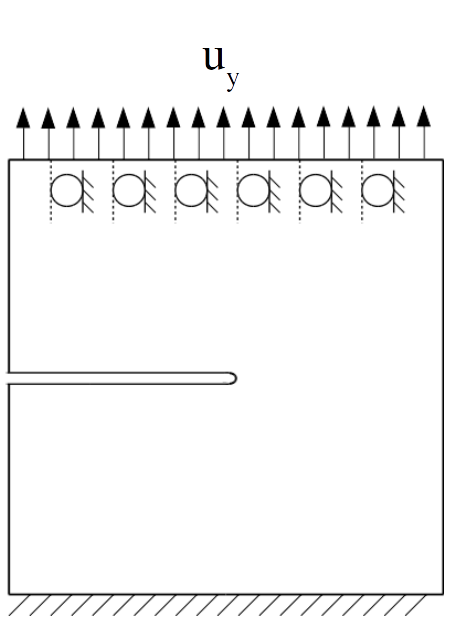
\includegraphics[width=0.8\textwidth,scale=0.5]{Chapter4/figures/mode1_bcs}
    \caption{}
    \label{fig: Chapter4/mode1_bcs}
  \end{subfigure}
  \hspace{0.03\textwidth}
  \begin{subfigure}[b]{0.19\textwidth}
    \centering
    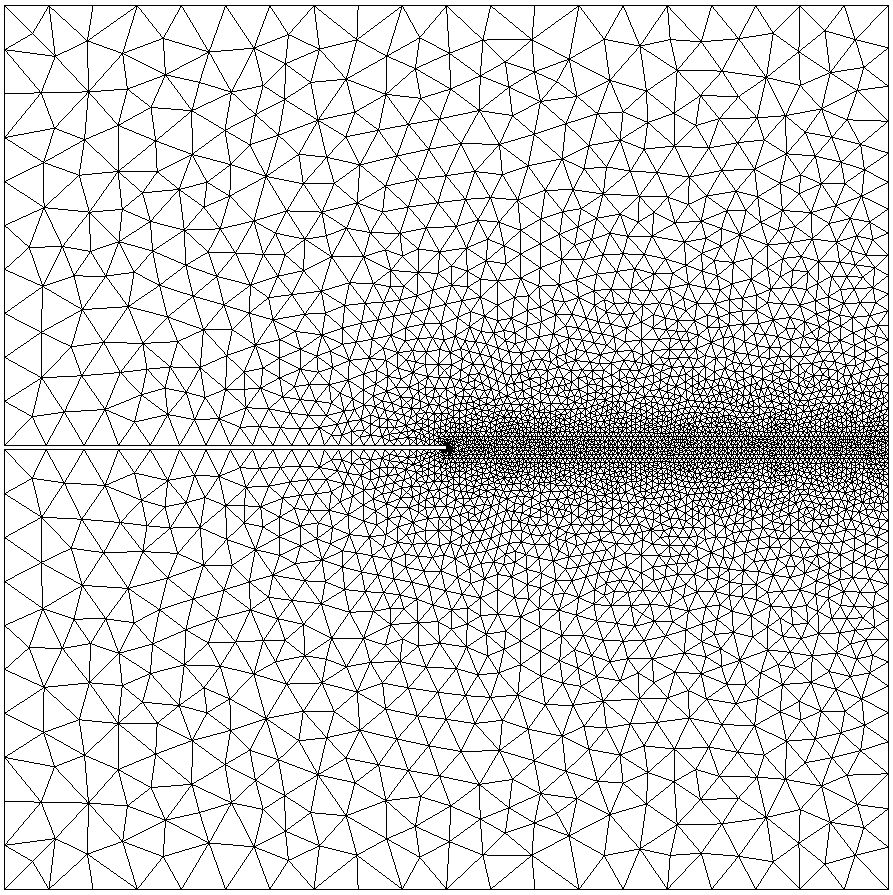
\includegraphics[width=\textwidth]{Chapter4/figures/mode1_notch_mesh.png}
    \caption{}
    \label{fig: Chapter4/mode1_notch_mesh}
  \end{subfigure}
  \hspace{0.05\textwidth}
  \begin{subfigure}[b]{0.19\textwidth}
    \centering
    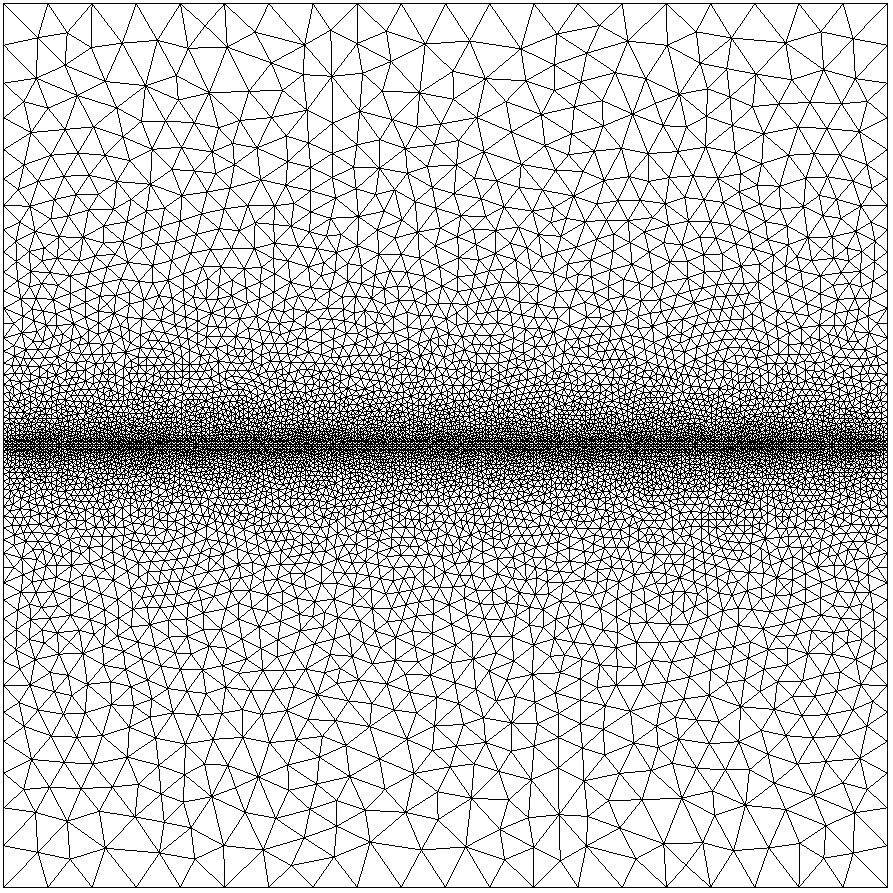
\includegraphics[width=\textwidth]{Chapter4/figures/mode1_initial_mesh.png}
    \caption{}
    \label{fig: Chapter4/mode1_initial_mesh}
  \end{subfigure}

  \begin{subfigure}[b]{0.25\textwidth}
    \centering
    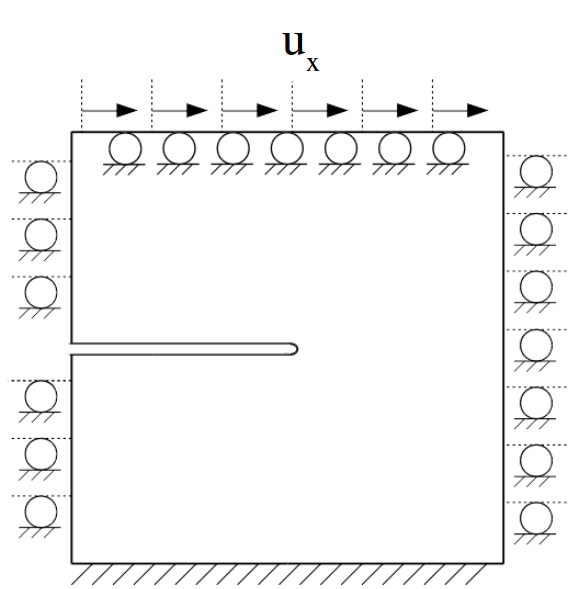
\includegraphics[width=\textwidth,scale=0.5]{Chapter4/figures/mode2_bcs.png}
    \caption{}
    \label{fig: Chapter4/mode2_bcs}
  \end{subfigure}
  \hspace{0.03\textwidth}
  \begin{subfigure}[b]{0.19\textwidth}
    \centering
    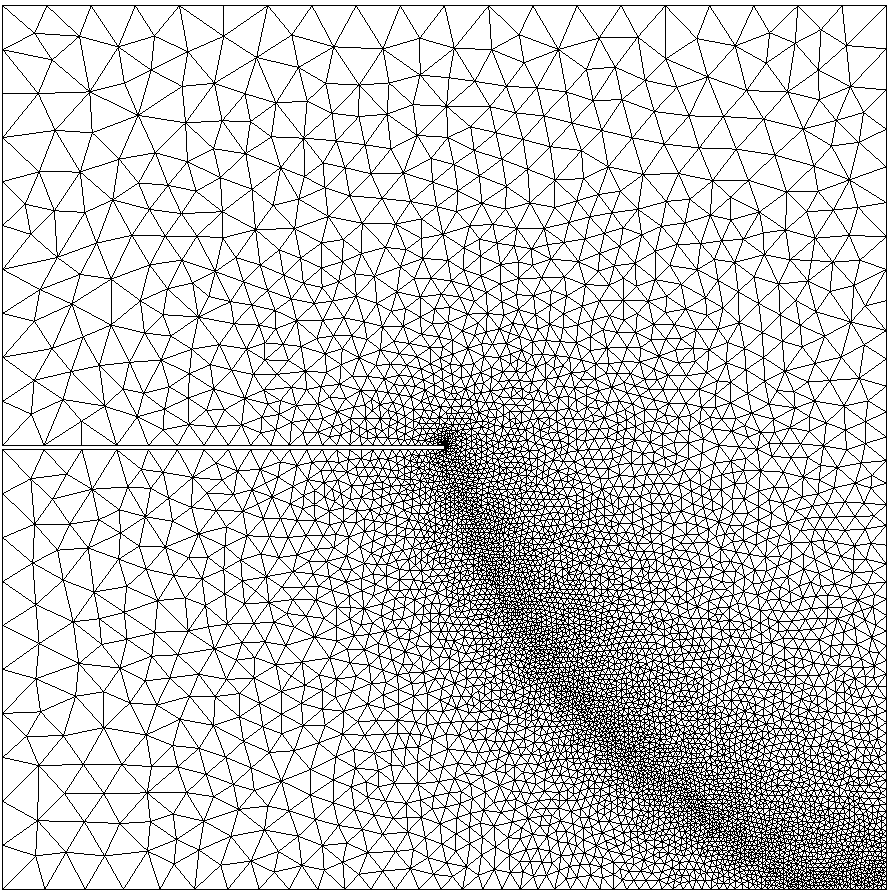
\includegraphics[width=\textwidth]{Chapter4/figures/mode2_notch_mesh.png}
    \caption{}
    \label{fig: Chapter4/mode2_notch_mesh}
  \end{subfigure}
  \hspace{0.05\textwidth}
  \begin{subfigure}[b]{0.19\textwidth}
    \centering
    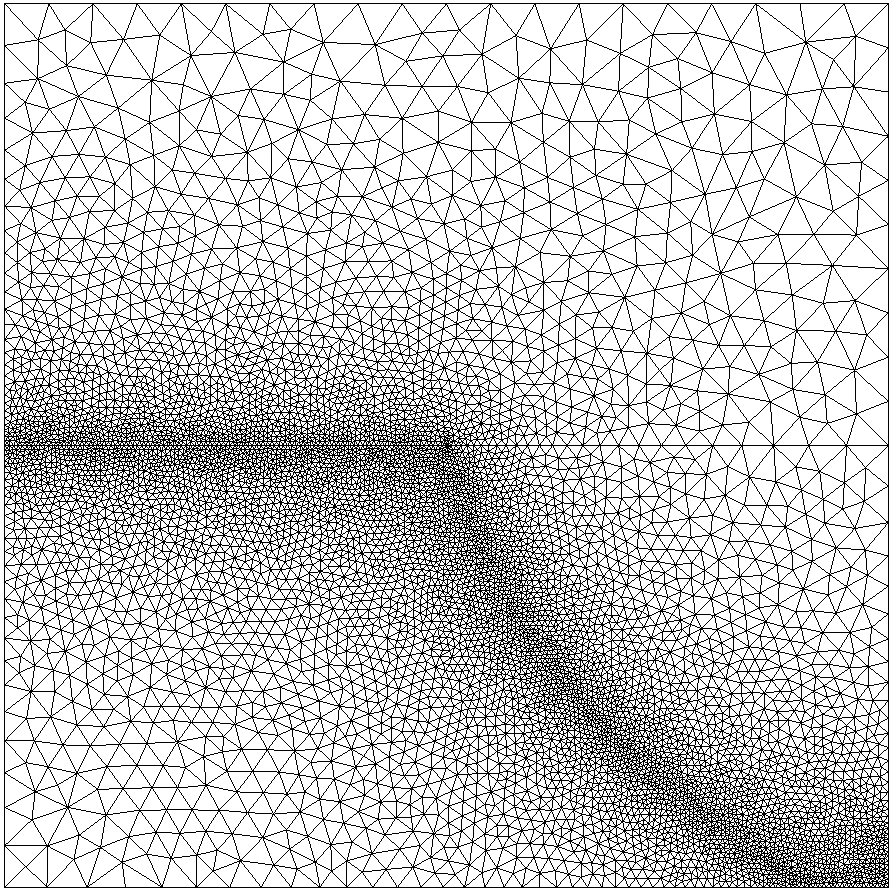
\includegraphics[width=\textwidth]{Chapter4/figures/mode2_initial_mesh.png}
    \caption{}
    \label{fig: Chapter4/mode2_initial_mesh}
  \end{subfigure}
  \caption{Boundary conditions of the plate with a pre-existing crack for (a) a mode I tension test and (d) a mode II shear test. Finite element meshes for the mode I calculations (b - c) and for the mode II calculations (e - f). For (b, e) the meshes have the initial crack geometry ``meshed-in'' while (c, f) have local refinement around the initial damage field. All meshes are pre-refined along the predicted crack-path with a characteristic element size of \SI{0.005}{\milli\meter}.}
  \label{fig: example/bcs}
\end{figure}


We examine two representations of the pre-existing crack. First, we use a ``geometric notch'' to represent the crack as shown in \Cref{fig: Chapter4/mode1_notch_mesh,fig: Chapter4/notched_plate_dimensions}. In this case, the traction-free boundary condition on the notch surfaces is satisfied in a weak sense.
The resulting phase fields as a function of boundary displacement are shown in \Cref{fig: Chapter4/mode1_notched_plate_damage_1,fig: Chapter4/mode1_notched_plate_damage_2,fig: Chapter4/mode1_notched_plate_damage_3}.
Only the phase fields obtained using the spectral decomposition are shown in the Figures.  Contours of the phase field obtained using the contact split with a threshold were found to be indistinguishable.

\begin{figure}[htb!]
  \begin{subfigure}[b]{0.23\textwidth}
    \centering
    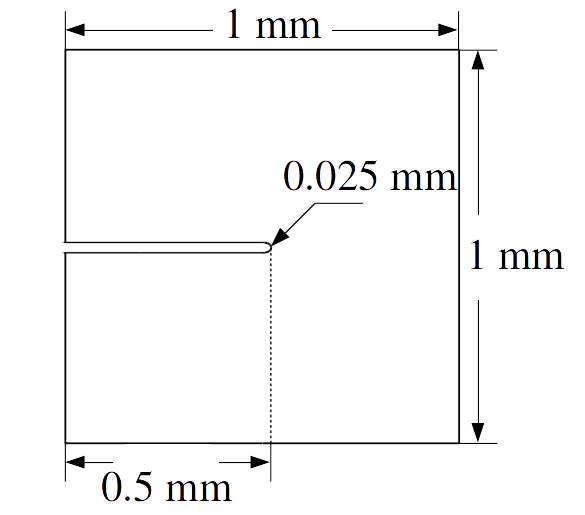
\includegraphics[width=\textwidth,scale=0.5]{Chapter4/figures/notched_plate_dimensions.png}
    \caption{}
    \label{fig: Chapter4/notched_plate_dimensions}
  \end{subfigure}
  \begin{subfigure}[b]{0.21\textwidth}
    \centering
    
\includegraphics[width=\textwidth,scale=0.5]{Chapter4/figures/notched_plate_initial.png}
    \caption{}
    \label{fig: Chapter4/mode1_notched_plate_damage_1}
  \end{subfigure}
  \begin{subfigure}[b]{0.21\textwidth}
    \centering
    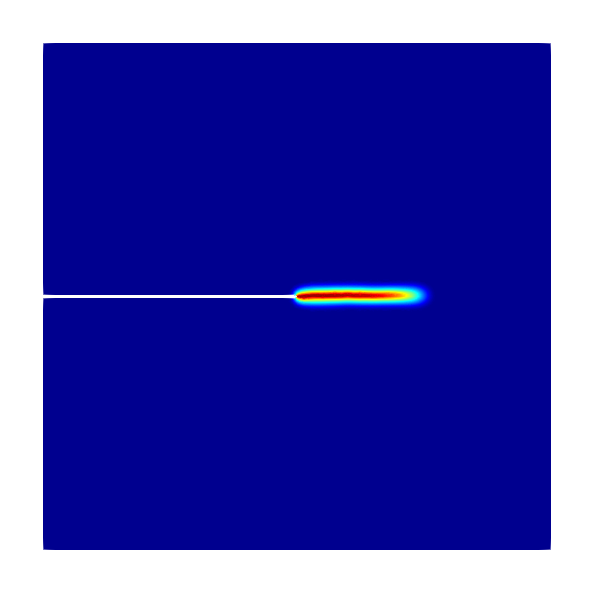
\includegraphics[width=\textwidth,scale=0.5]{Chapter4/figures/mode1_notched_plate_intermediate.png}
    \caption{}
    \label{fig: Chapter4/mode1_notched_plate_damage_2}
  \end{subfigure}
  \begin{subfigure}[b]{0.21\textwidth}
    \centering
    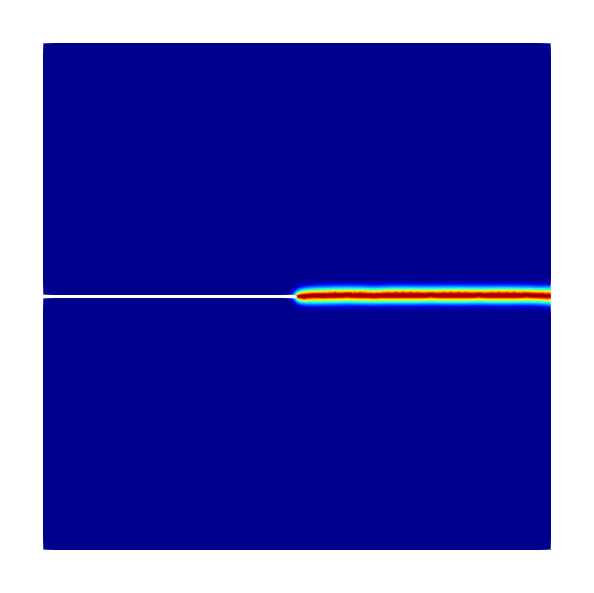
\includegraphics[width=\textwidth,scale=0.5]{Chapter4/figures/mode1_notched_plate_final.png}
    \caption{}
    \label{fig: Chapter4/mode1_notched_plate_damage_3}
  \end{subfigure}
  \begin{subfigure}[b]{0.06\textwidth}
    \centering
    \caption*{d}
    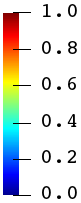
\includegraphics[width=\textwidth]{Chapter4/figures/jet_vertical.png}
    \vspace{0.15in}
  \end{subfigure}
  \caption[Edge-notched specimen loaded in tension with initial crack represented by a geometric notch with a rounded corner.]{Edge-notched specimen loaded in tension with initial crack represented by a geometric notch with a rounded corner.  (a) Dimensions of the notched plate. Damage $d$ at (b) $u_y = \SI{0}{\milli\meter}$, (c) $u_y = \SI{0.0048}{\milli\meter}$, (d) $u_y = \SI{0.006}{\milli\meter}$.}
  \label{fig: Chapter4/mode1_notched_plate}
\end{figure}


Secondly, we use an initial phase field $d(t = 0) = d_0$ to represent the initial crack, where $d_0$ is given by:
\begin{align}
  d_0(\btX)   & =                                            
  \begin{cases}
    \left( 1-\dfrac{\tau(\btX)}{2l} \right)^2, \quad \tau(\btX) \leqslant 2l \\
    0, \quad  \tau(\btX) > 2l
  \end{cases} \label{eq: mode1 initial damage} \\
  \mbox{with} &                                              \\
  \tau(\btX)  & =                                            
  \begin{cases}
    \left\vert \btX\cdot\bs{e}_2 \right\vert, \quad \btX\cdot\bs{e}_1 \leqslant 0, \\
    \norm{\btX}, \quad \btX\cdot\bs{e}_1 > 0,
  \end{cases}
\end{align}
with an origin for the coordinate system at the center of the plate. The initial phase field is resolved using the locally refined mesh of linear triangular elements shown in \Cref{fig: Chapter4/mode1_initial_mesh}. The resulting initial phase field is shown in \Cref{fig: Chapter4/intact_plate_initial}.  Once again, the contour plots of the phase field obtained using a spectral decomposition and the contact split were found to be indistinguishable.

\begin{figure}[htb!]
  \hspace{0.015\textwidth}
  \begin{subfigure}[b]{0.21\textwidth}
    \centering
    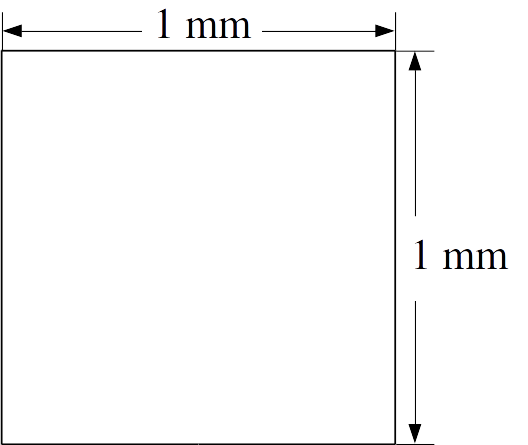
\includegraphics[width=\textwidth,scale=0.5]{Chapter4/figures/intact_plate_dimensions.png}
    \vspace{-0.03\textwidth}
    \caption{}
  \end{subfigure}
  \begin{subfigure}[b]{0.21\textwidth}
    \centering
    
\includegraphics[width=\textwidth,scale=0.5]{Chapter4/figures/intact_plate_initial.png}
    \caption{}
    \label{fig: Chapter4/intact_plate_initial}
  \end{subfigure}
  \begin{subfigure}[b]{0.21\textwidth}
    \centering
    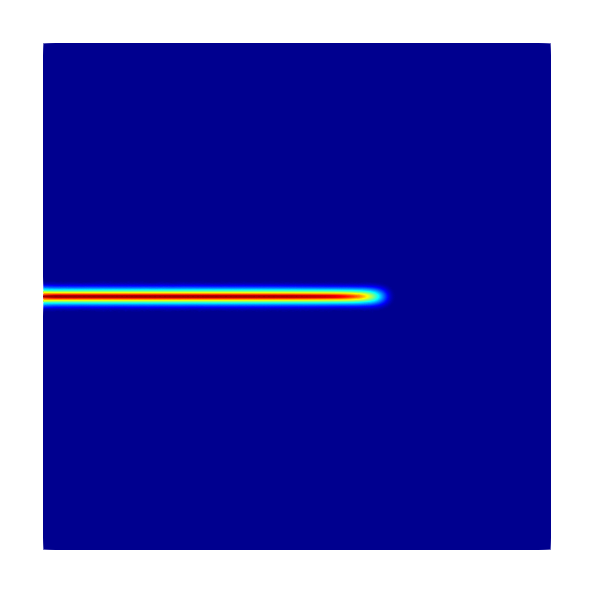
\includegraphics[width=\textwidth,scale=0.5]{Chapter4/figures/mode1_intact_plate_intermediate.png}
    \caption{}
  \end{subfigure}
  \begin{subfigure}[b]{0.21\textwidth}
    \centering
    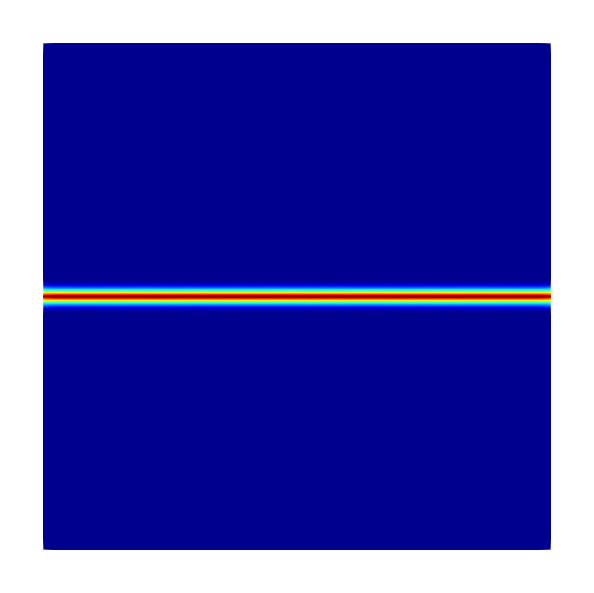
\includegraphics[width=\textwidth,scale=0.5]{Chapter4/figures/mode1_intact_plate_final.png}
    \caption{}
  \end{subfigure}
  \begin{subfigure}[b]{0.06\textwidth}
    \centering
    \caption*{d}
    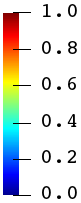
\includegraphics[width=\textwidth]{Chapter4/figures/jet_vertical.png}
    \vspace{0.15in}
  \end{subfigure}
  \caption[Edge-notched specimen loaded in tension  with initial crack represented by a phase field.]{ Edge-notched specimen loaded in tension  with initial crack represented by a phase field.  (a) Dimensions of the intact plate. The  Damage $d$ at (b) $u_y = \SI{0}{\milli\meter}$ (c) $u_y = \SI{0.0048}{\milli\meter}$ (d) $u_y = \SI{0.006}{\milli\meter}$. }
  \label{fig: Chapter4/mode1_intact_plate}
\end{figure}


Plots of the vertical component of the reaction force at the top boundary of the plate versus the prescribed y--displacement are shown in \Cref{fig: Chapter4/mode1_force_displacement}, for both representations of the initial crack and split strategies.  The reaction force is nondimensionalized with respect to the critical strength and the plate thickness, i.e. $f_y^* = f_y / (\sigma_c t)$, and the displacement is nondimensionalized by $u_y^* = u_y / a$, where $a$ is the side length of the square plate.  As expected, the contact split does not affect the material response in the uniaxial loading case (\Cref{fig: Chapter4/mode1_force_displacement_compare_decomposition}), and the results appear to be relatively insensitive to the choice of threshold for switching between the spectral split and the contact split (\Cref{fig: Chapter4/mode1_force_displacement_compare_dcritical}).

\begin{figure}[htb!]
  \centering
  \begin{subfigure}{0.47\textwidth}
    \centering
    \tikzsetnextfilenamesafe{Chapter4/mode1_force_displacement_compare_decomposition}
    \begin{tikzpicture}
      \begin{axis}[
          cycle list name=exotic,
          width=\textwidth,
          height=1.2\textwidth,
          xlabel=$u_y^*$,ylabel=$f_y^*$,
          xmin=0,
          xmax=0.006,
          ymin=0,
          ymax=0.45,
          legend style={at={(0.05,0.95)},anchor=north west},
          legend style={nodes={scale=0.8, transform shape}},
          legend style={draw=none, fill=none},
          legend style={cells={align=left}},
          every axis plot/.append style={thick}
        ]
        \addplot +[mark=none] table[x expr=\thisrowno{2},y expr=\thisrowno{1}*20.9036/2500] {Chapter4/data/mode1_notched_plate_spectral.csv};
        \addplot +[mark=none] table[x expr=\thisrowno{2},y expr=\thisrowno{1}*20.9036/2500] {Chapter4/data/mode1_notched_plate_odd_0.6.csv};
        \addplot +[mark=none] table[x expr=\thisrowno{2},y expr=\thisrowno{1}*20.9036/2500] {Chapter4/data/mode1_intact_plate_spectral.csv};
        \addplot +[mark=none] table[x expr=\thisrowno{2},y expr=\thisrowno{1}*20.9036/2500] {Chapter4/data/mode1_intact_plate_odd_0.6.csv};
        \legend{geometric notch\text{,} spectral split,geometric notch\text{,} spectral split \\ $+$ contact split,initial damage\text{,} spectral split,initial damage\text{,} spectral split \\ $+$ contact split}
      \end{axis}
    \end{tikzpicture}
    \caption{}
    \label{fig: Chapter4/mode1_force_displacement_compare_decomposition}
  \end{subfigure}
  \begin{subfigure}{0.47\textwidth}
    \centering
    \tikzsetnextfilenamesafe{Chapter4/mode1_force_displacement_compare_dcritical}
    \begin{tikzpicture}
      \begin{axis}[
          cycle list name=exotic,
          width=\textwidth,
          height=1.2\textwidth,
          xlabel=$u_y^*$,ylabel=$f_y^*$,
          xmin=0,
          xmax=0.006,
          ymin=0,
          ymax=0.45,
          legend style={at={(0.05,0.95)},anchor=north west},
          legend style={nodes={scale=0.8, transform shape}},
          legend style={draw=none, fill=none},
          legend cell align={left},
          every axis plot/.append style={thick}
        ]
        \addplot +[mark=none] table[x expr=\thisrowno{2},y expr=\thisrowno{1}*20.9036/2500] {Chapter4/data/mode1_notched_plate_odd_0.4.csv};
        \addplot +[mark=none] table[x expr=\thisrowno{2},y expr=\thisrowno{1}*20.9036/2500] {Chapter4/data/mode1_notched_plate_odd_0.6.csv};
        \addplot +[mark=none] table[x expr=\thisrowno{2},y expr=\thisrowno{1}*20.9036/2500] {Chapter4/data/mode1_notched_plate_odd_0.8.csv};
        \addplot +[mark=none] table[x expr=\thisrowno{2},y expr=\thisrowno{1}*20.9036/2500] {Chapter4/data/mode1_intact_plate_odd_0.4.csv};
        \addplot +[mark=none] table[x expr=\thisrowno{2},y expr=\thisrowno{1}*20.9036/2500] {Chapter4/data/mode1_intact_plate_odd_0.6.csv};
        \addplot +[mark=none] table[x expr=\thisrowno{2},y expr=\thisrowno{1}*20.9036/2500] {Chapter4/data/mode1_intact_plate_odd_0.8.csv};
        \legend{geometric notch $d_c=0.4$,geometric notch $d_c=0.6$,geometric notch $d_c=0.8$,initial damage $d_c=0.4$,initial damage $d_c=0.6$,initial damage $d_c=0.8$}
      \end{axis}
    \end{tikzpicture}
    \caption{}
    \label{fig: Chapter4/mode1_force_displacement_compare_dcritical}
  \end{subfigure}
  \caption[Mode I force--displacement curves.]{ Mode I force--displacement curves obtained using (a) the spectral decomposition with two representations of the pre-existing crack (b) a spectral decomposition in conjunction with the contact split with different critical damage threshold on two representations of the pre-existing crack. }
  \label{fig: Chapter4/mode1_force_displacement}
\end{figure}


%%%%%%%%%%%%%%%%%%%%%%%%%%%%%%%%%%%%%%%%%%%%%%%%%%%%%%%%%%%%%%%%%%%%%%%%%%%%%%%%%%%%%%%%%%%
%%%%%%%%%%%%%%%%%%%%%%%%%%%%%%%%%%%%%%%%%%%%%%%%%%%%%%%%%%%%%%%%%%%%%%%%%%%%%%%%%%%%%%%%%%%
\subsection{Mode II: Edge-Notched Shear Test}

The effect of the proposed energy split becomes readily apparent when the loading case is dominated by in--plane or out--of--plane shear. Let us consider the same edge--notched thick plate as in the last section, but subjected to a different loading. A schematic of the boundary conditions for this case and the corresponding meshes are shown in \Cref{fig: Chapter4/mode2_bcs,fig: Chapter4/mode2_notch_mesh,fig: Chapter4/mode2_initial_mesh}.

\begin{figure}[htb!]
  \begin{subfigure}[b]{0.23\textwidth}
    \centering
    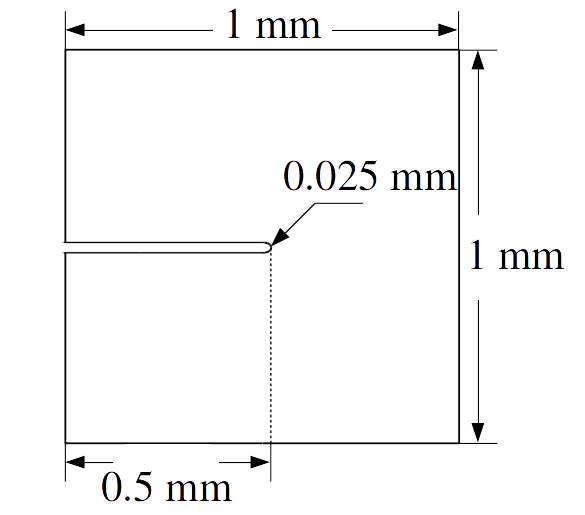
\includegraphics[width=\textwidth,scale=0.5]{Chapter4/figures/notched_plate_dimensions.png}
    \caption{}
  \end{subfigure}
  \begin{subfigure}[b]{0.21\textwidth}
    \centering
    
\includegraphics[width=\textwidth,scale=0.5]{Chapter4/figures/notched_plate_initial.png}
    \caption{}
  \end{subfigure}
  \begin{subfigure}[b]{0.21\textwidth}
    \centering
    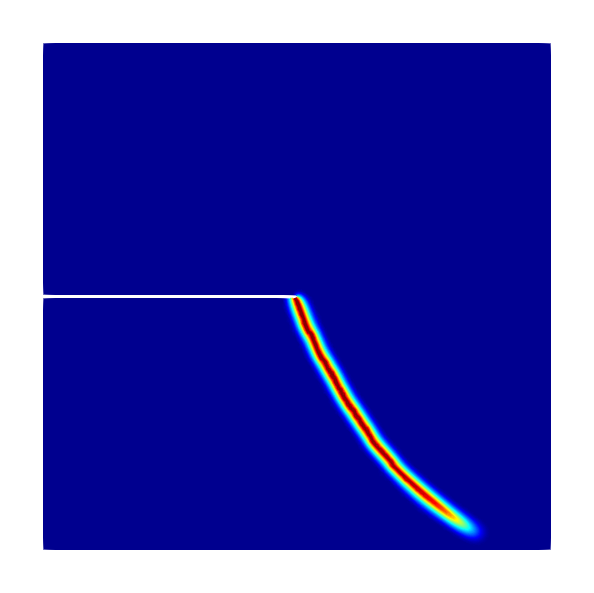
\includegraphics[width=\textwidth,scale=0.5]{Chapter4/figures/mode2_notched_plate_spectral_intermediate.png}
    \caption{}
    \label{fig: Chapter4/mode2_notched_plate_spectral_intermediate}
  \end{subfigure}
  \begin{subfigure}[b]{0.21\textwidth}
    \centering
    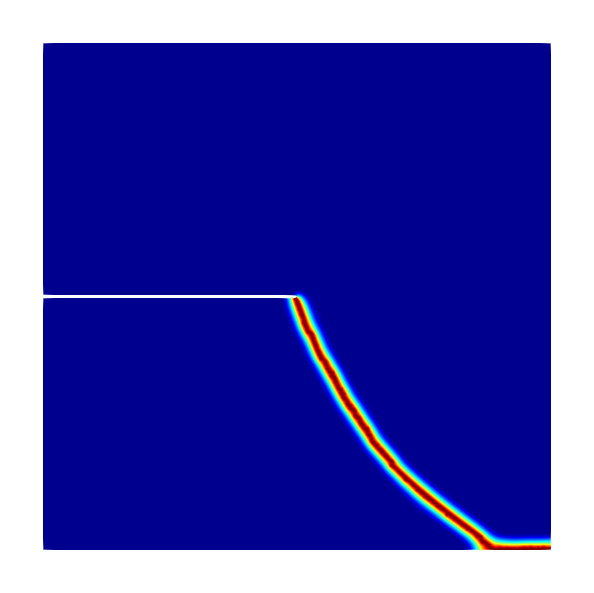
\includegraphics[width=\textwidth,scale=0.5]{Chapter4/figures/mode2_notched_plate_spectral_final.png}
    \caption{}
    \label{fig: Chapter4/mode2_notched_plate_spectral_final}
  \end{subfigure}
  \begin{subfigure}[b]{0.06\textwidth}
    \centering
    \caption*{d}
    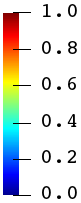
\includegraphics[width=\textwidth]{Chapter4/figures/jet_vertical.png}
    \vspace{0.15in}
  \end{subfigure}
  
  \hspace{0.015\textwidth}
  \begin{subfigure}[b]{0.21\textwidth}
    \centering
    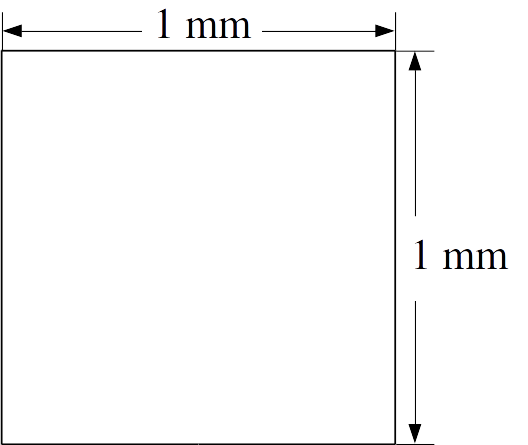
\includegraphics[width=\textwidth,scale=0.5]{Chapter4/figures/intact_plate_dimensions.png}
    \vspace{-0.03\textwidth}
    \caption{}
  \end{subfigure}
  \begin{subfigure}[b]{0.21\textwidth}
    \centering
    
\includegraphics[width=\textwidth,scale=0.5]{Chapter4/figures/intact_plate_initial.png}
    \caption{}
  \end{subfigure}
  \begin{subfigure}[b]{0.21\textwidth}
    \centering
    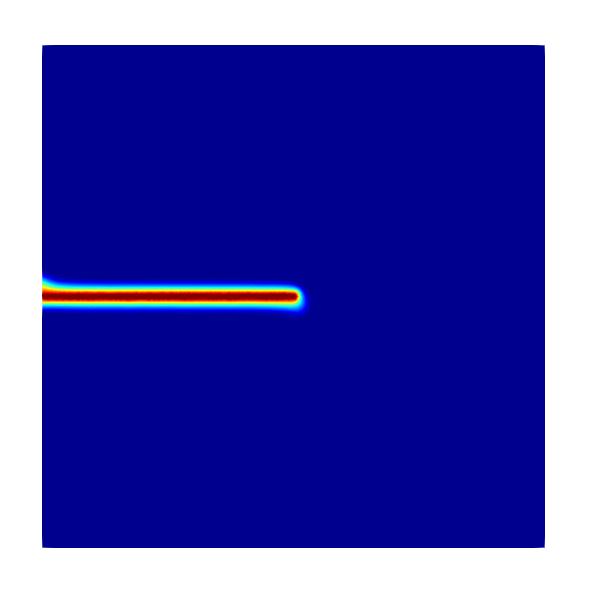
\includegraphics[width=\textwidth,scale=0.5]{Chapter4/figures/mode2_intact_plate_spectral_intermediate.png}
    \caption{}
    \label{fig: Chapter4/mode2_intact_plate_spectral_intermediate}
  \end{subfigure}
  \begin{subfigure}[b]{0.21\textwidth}
    \centering
    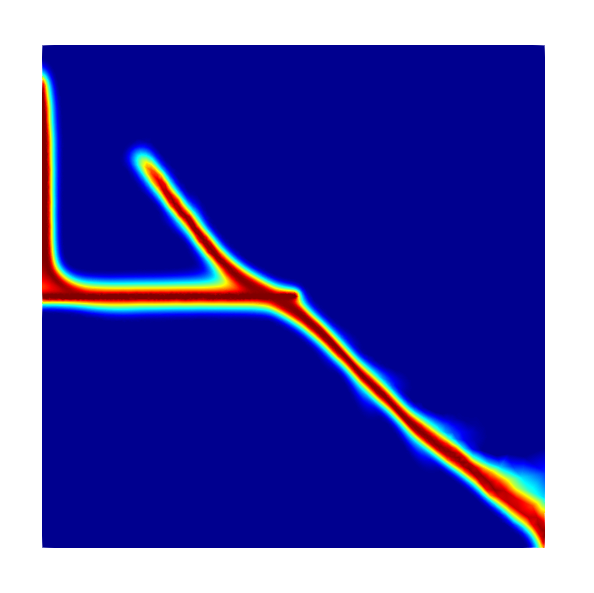
\includegraphics[width=\textwidth,scale=0.5]{Chapter4/figures/mode2_intact_plate_spectral_final.png}
    \caption{}
    \label{fig: Chapter4/mode2_intact_plate_spectral_final}
  \end{subfigure}
  \begin{subfigure}[b]{0.06\textwidth}
    \centering
    \caption*{d}
    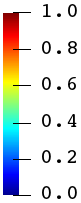
\includegraphics[width=\textwidth]{Chapter4/figures/jet_vertical.png}
    \vspace{0.15in}
  \end{subfigure}
  
  \hspace{0.015\textwidth}
  \begin{subfigure}[b]{0.21\textwidth}
    \centering
    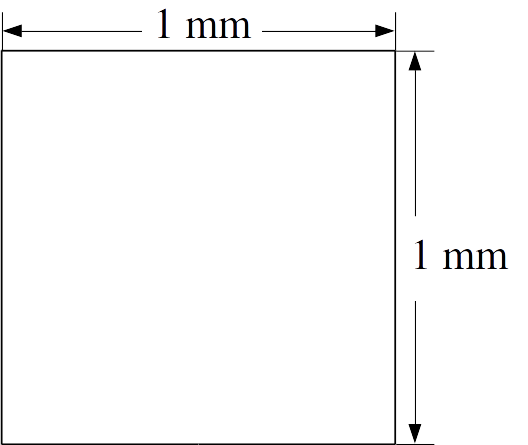
\includegraphics[width=\textwidth,scale=0.5]{Chapter4/figures/intact_plate_dimensions.png}
    \vspace{-0.03\textwidth}
    \caption{}
  \end{subfigure}
  \begin{subfigure}[b]{0.21\textwidth}
    \centering
    
\includegraphics[width=\textwidth,scale=0.5]{Chapter4/figures/intact_plate_initial.png}
    \caption{}
  \end{subfigure}
  \begin{subfigure}[b]{0.21\textwidth}
    \centering
    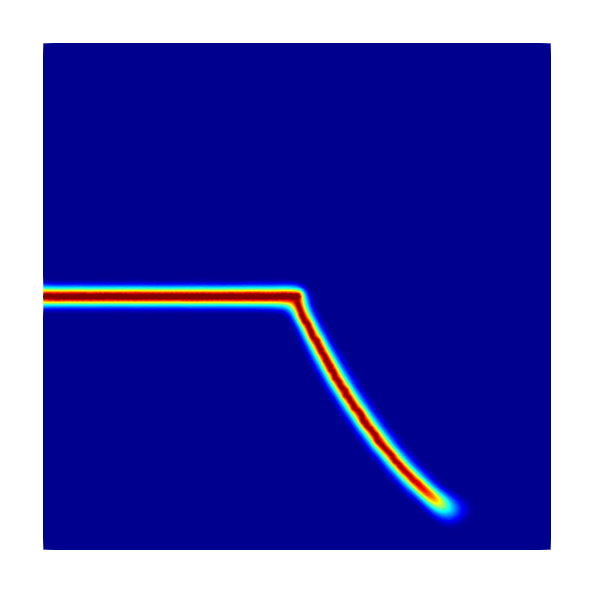
\includegraphics[width=\textwidth,scale=0.5]{Chapter4/figures/mode2_intact_plate_odd_intermediate.png}
    \caption{}
    \label{fig: Chapter4/mode2_intact_plate_odd_intermediate}
  \end{subfigure}
  \begin{subfigure}[b]{0.21\textwidth}
    \centering
    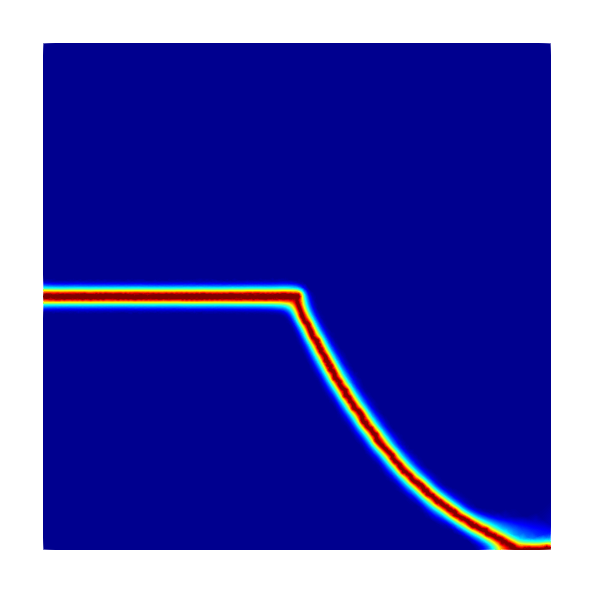
\includegraphics[width=\textwidth,scale=0.5]{Chapter4/figures/mode2_intact_plate_odd_final.png}
    \caption{}
    \label{fig: Chapter4/mode2_intact_plate_odd_final}
  \end{subfigure}
  \begin{subfigure}[b]{0.06\textwidth}
    \centering
    \caption*{d}
    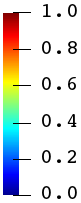
\includegraphics[width=\textwidth]{Chapter4/figures/jet_vertical.png}
    \vspace{0.15in}
  \end{subfigure}
  \caption[The crack paths for the Mode-II test.]{The crack paths obtained using (a-d) the spectral decomposition on a geometrically notched plate, (e-h) the spectral decomposition with an initial phase field $d_0$ \eqref{eq: mode1 initial damage} representing the initial crack, and (i-l) the contact split with an initial phase field. Snapshots of crack paths are shown at (b,f,j) $u_x = \SI{0}{\milli\meter}$, (c,g,k) $u_x = \SI{0.0109}{\milli\meter}$, and (d,h,l) $u_x = \SI{0.02}{\milli\meter}$. }
  \label{fig: Chapter4/mode2_crack_path}
\end{figure}


\begin{figure}[htb!]
  \centering
  \begin{subfigure}{0.47\textwidth}
    \centering
    \tikzsetnextfilenamesafe{Chapter4/mode2_force_displacement_compare_decomposition}
    \begin{tikzpicture}
      \begin{axis}[
          cycle list name=exotic,
          width=\textwidth,
          height=1.5\textwidth,
          xlabel=$u_x^*$,ylabel=$f_x^*$,
          xmin=0,
          xmax=0.02,
          ymin=0,
          ymax=0.35,
          legend style={
              at={(0.05,0.98)},
              anchor=north west,
              nodes={scale=0.8, transform shape},
              fill=none,
              draw=none,
              text opacity=1,
              cells={align=left}
            },
          legend cell align={left},
          every axis plot/.append style={thick},
          yticklabel style={
              /pgf/number format/fixed
            }
        ]
        \addplot +[mark=none] table[x expr=\thisrowno{2},y expr=\thisrowno{1}*20.9036/2500] {Chapter4/data/mode2_notched_plate_spectral.csv};
        \addplot +[mark=none] table[x expr=\thisrowno{2},y expr=\thisrowno{1}*20.9036/2500] {Chapter4/data/mode2_notched_plate_odd_0.6.csv};
        \addplot +[mark=none] table[x expr=\thisrowno{2},y expr=\thisrowno{1}*20.9036/2500] {Chapter4/data/mode2_intact_plate_odd_0.6.csv};
        \legend{geometric notch\text{,} spectral split,geometric notch\text{,} spectral split \\ $+$ contact split,initial damage\text{,} spectral split \\ $+$ contact split}
      \end{axis}
    \end{tikzpicture}
    \caption{}
    \label{fig: Chapter4/mode2_force_displacement_compare_decomposition}
  \end{subfigure}
  \begin{subfigure}{0.47\textwidth}
    \centering
    \tikzsetnextfilenamesafe{Chapter4/mode2_force_displacement_compare_dcrit}
    \begin{tikzpicture}
      \begin{axis}[
          cycle list name=exotic,
          width=\textwidth,
          height=1.5\textwidth,
          xlabel=$u_x^*$,ylabel=$f_x^*$,
          xmin=0,
          xmax=0.02,
          ymin=0,
          ymax=0.35,
          legend style={
              at={(0.98,0.98)},
              anchor=north east,
              nodes={scale=0.8, transform shape},
              fill=none,
              draw=none,
              text opacity=1
            },
          legend cell align={left},
          every axis plot/.append style={thick},
          yticklabel style={
              /pgf/number format/fixed
            }
        ]
        \addplot +[mark=none] table[x expr=\thisrowno{2},y expr=\thisrowno{1}*20.9036/2500] {Chapter4/data/mode2_notched_plate_odd_0.2.csv};
        \addplot +[mark=none] table[x expr=\thisrowno{2},y expr=\thisrowno{1}*20.9036/2500] {Chapter4/data/mode2_notched_plate_odd_0.4.csv};
        \addplot +[mark=none] table[x expr=\thisrowno{2},y expr=\thisrowno{1}*20.9036/2500] {Chapter4/data/mode2_notched_plate_odd_0.6.csv};
        \addplot +[mark=none] table[x expr=\thisrowno{2},y expr=\thisrowno{1}*20.9036/2500] {Chapter4/data/mode2_notched_plate_odd_0.8.csv};
        \addplot +[mark=none] table[x expr=\thisrowno{2},y expr=\thisrowno{1}*20.9036/2500] {Chapter4/data/mode2_intact_plate_odd_0.2.csv};
        \addplot +[mark=none] table[x expr=\thisrowno{2},y expr=\thisrowno{1}*20.9036/2500] {Chapter4/data/mode2_intact_plate_odd_0.4.csv};
        \addplot +[mark=none] table[x expr=\thisrowno{2},y expr=\thisrowno{1}*20.9036/2500] {Chapter4/data/mode2_intact_plate_odd_0.6.csv};
        \addplot +[mark=none] table[x expr=\thisrowno{2},y expr=\thisrowno{1}*20.9036/2500] {Chapter4/data/mode2_intact_plate_odd_0.8.csv};
        \legend{geometric notch $d_c=0.2$,geometric notch $d_c=0.4$,geometric notch $d_c=0.6$,geometric notch $d_c=0.8$,initial damage $d_c=0.2$,initial damage $d_c=0.4$,initial damage $d_c=0.6$,initial damage $d_c=0.8$}
      \end{axis}
    \end{tikzpicture}
    \caption{}
    \label{fig: Chapter4/mode2_force_displacement_compare_dcrit}
  \end{subfigure}
  \caption[Mode II force--displacement curves.]{ Mode II force--displacement curves obtained using (a) spectral decomposition with two representations of the initial crack (b) spectral decomposition in conjunction with the contact split with different critical damage threshold on two representations of the initial crack. }
  \label{fig: Chapter4/mode2_force_displacement}
\end{figure}


Once again, the effect of the contact split is examined by comparing the results using two different representations of the initial crack, as shown in \Cref{fig: Chapter4/mode2_crack_path} and \Cref{fig: Chapter4/mode2_force_displacement_compare_decomposition}.
Simulations that rely solely on the spectral decomposition result in dramatically different crack paths (\Cref{fig: Chapter4/mode2_notched_plate_spectral_intermediate,fig: Chapter4/mode2_notched_plate_spectral_final,fig: Chapter4/mode2_intact_plate_spectral_intermediate,fig: Chapter4/mode2_intact_plate_spectral_final})
and force-displacement responses (\Cref{fig: Chapter4/mode2_force_displacement_compare_decomposition}). We note that after the initial decay following a horizontal displacement of $u_x = 1.0\times 10^{-2}$mm, the force for the geometric notch with the spectral decomposition begins to rise.  Even though the phase field completely separates the plate into two sections, the force continues to increase.  This is because the spectral decomposition does not prevent all traction from being transmitted across a fully damaged surface.

In contrast, when the traction-free condition is enforced using the contact split, the crack paths (\Cref{fig: Chapter4/mode2_notched_plate_spectral_intermediate,fig: Chapter4/mode2_notched_plate_spectral_final,fig: Chapter4/mode2_intact_plate_odd_intermediate,fig: Chapter4/mode2_intact_plate_odd_final}) as well as the force-displacement curves (\Cref{fig: Chapter4/mode2_force_displacement_compare_dcrit}) are similar for both representations of the pre--existing crack.
Notably in this case, the force at the boundary decays completely to zero as the plate is separated in two by the phase field.   As shown in \Cref{fig: Chapter4/mode2_force_displacement_compare_dcrit}, the results are also relatively insensitive to the particular choice of threshold for the contact split.

We note that if the threshold is selected to be too high (e.g.\ $d_{\critical} \ge 0.8$) a small upward perturbation in the force-displacement curve can be observed, shortly after a horizontal displacement of $u_x = 1.0\times 10^{-2}$mm.  The brief increase is due to the fact that the band of damage wherein the contact split is applied is too small, and some traction can still be transmitted across the fully damaged band.  Essentially, there are elements capturing the peak phase field wherein some quadrature points are below the threshold while others are above it.
While further mesh refinement can remove this artifact, in practice we employ meshes that sufficiently capture the phase-field regularization, wherein $ 2 l / h^e = 5$.  Given this level of mesh refinement and typical damage profiles, we anticipate that a threshold of $d_{\critical} = 0.6$ is sufficient to prevent any such artifacts.  As such, we employ a threshold of $d_{\critical} = 0.6$ for all subsequent problems.

%%%%%%%%%%%%%%%%%%%%%%%%%%%%%%%%%%%%%%%%%%%%%%%%%%%%%%%%%%%%%%%%%%%%%%%%%%%%%%%%%%%%%%%%%%%
%%%%%%%%%%%%%%%%%%%%%%%%%%%%%%%%%%%%%%%%%%%%%%%%%%%%%%%%%%%%%%%%%%%%%%%%%%%%%%%%%%%%%%%%%%%
\subsection{Crack Propagation Under Biaxial Tension}

We now examine a problem in which a thin plate  with initial imperfections is subject to biaxial tension.  Plane-stress conditions are assumed to hold. The plate geometry and boundary conditions are summarized in \Cref{fig: Chapter4/biaxial_dimensions}, and the initial phase field representing two imperfections is shown in \Cref{fig: Chapter4/biaxial_initial}.  Periodic boundary conditions are assumed on all sides.

Using property values that are representative of a typical clay specimen, the plate is assumed to be composed of a material with a Young's modulus $E$ of \SI{4}{\mega\pascal}, a Poisson's ratio $\nu$ of 0.2, a fracture toughness $\Gc$ of \SI{27}{\kilo\joule\per\square\meter}, and a critical fracture energy $\psi_c$ of \SI{30}{\joule\per\square\meter}.

The governing equation for the mechanical problem in this case is given by:
\begin{align}
  \label{eq:biaxial}
  \nabla \cdot \left( \widetilde{\stress} + \sigma_0\bs{I} \right) = 0 ,
\end{align}
where $\sigma_0$ is a scalar-valued function that varies temporally and serves to model the drying process. The initial stress $\sigma_0\bs{I}$ is equivalent to an inelastic eigen-strain, i.e.\ $\strain_0 = \mathbb{S}:(\sigma_0\bs{I})$, where $\mathbb{S}$ is the compliance tensor.

With a view towards nondimensionalization, as will be discussed in \Cref{section: Chapter4/examples/1D}, the fracture driving force may be nondimensionalized as
\begin{align}
  \mathcal{D}^* = \sqrt{\dfrac{(1-\nu^2)a}{E\Gc}}\sigma_0,
\end{align}
where $a$ is a characteristic size for the domain.  Here, we choose it to be the width of the plate.

\begin{figure}[htb!]
  \centering
  \begin{subfigure}[b]{0.38\textwidth}
    \centering
    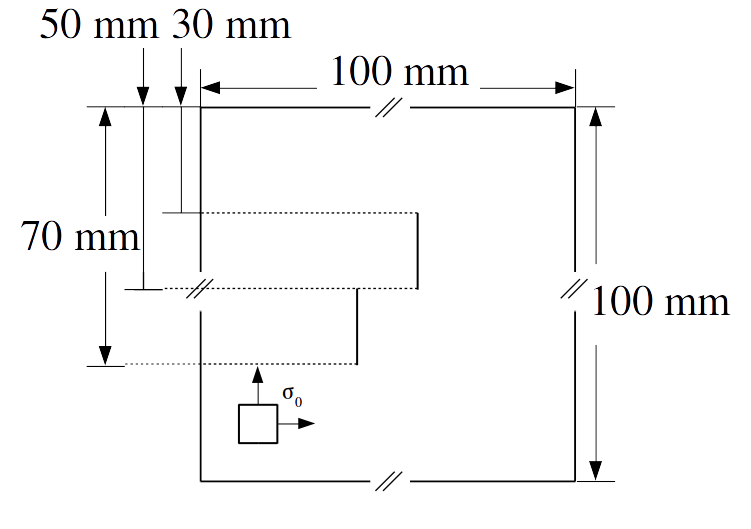
\includegraphics[width=\textwidth,scale=0.5]{Chapter4/figures/biaxial_dimensions.png}
    \caption{}
    \label{fig: Chapter4/biaxial_dimensions}
  \end{subfigure}
  \begin{subfigure}[b]{0.325\textwidth}
    \centering
    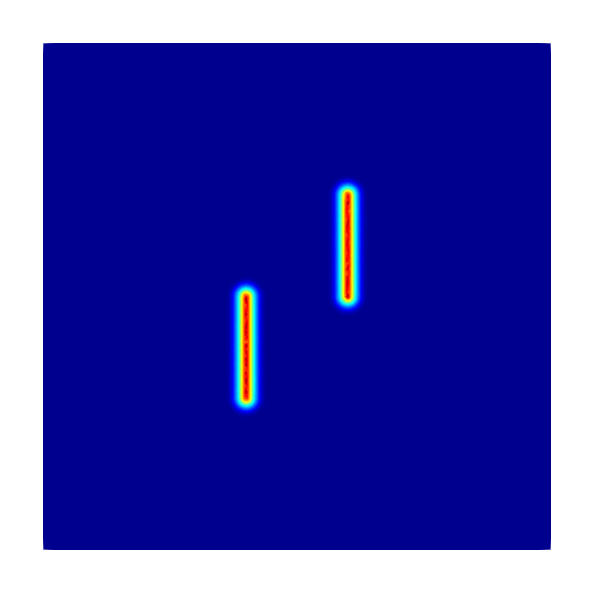
\includegraphics[width=0.73\textwidth,scale=0.5]{Chapter4/figures/biaxial_initial.png}
    \caption{}
    \label{fig: Chapter4/biaxial_initial}
  \end{subfigure}
  \begin{subfigure}[b]{0.07\textwidth}
    \centering
    \caption*{d}
    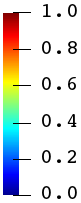
\includegraphics[width=\textwidth]{Chapter4/figures/jet_vertical.png}
    \vspace{0.15in}
  \end{subfigure}
  \caption{(a) Dimensions and boundary conditions of a thin plate with two parallel initial cracks. (b) The initial cracks are represented by an initial phase field.}
  \label{fig: Chapter4/biaxial_schematic}
\end{figure}


We now compare simulation results obtained using three strain energy split techniques: a no-split approach, the spectral split, and the contact split. The phase fields obtained using the three different split techniques are shown in \Cref{fig: Chapter4/biaxial_crack_path} at representative magnitudes of the dimensionless driving force.

% !TEX root = ../../main.tex

\begin{figure}[htb!]
  \centering
  \begin{subfigure}[b]{0.23\textwidth}
    \centering
    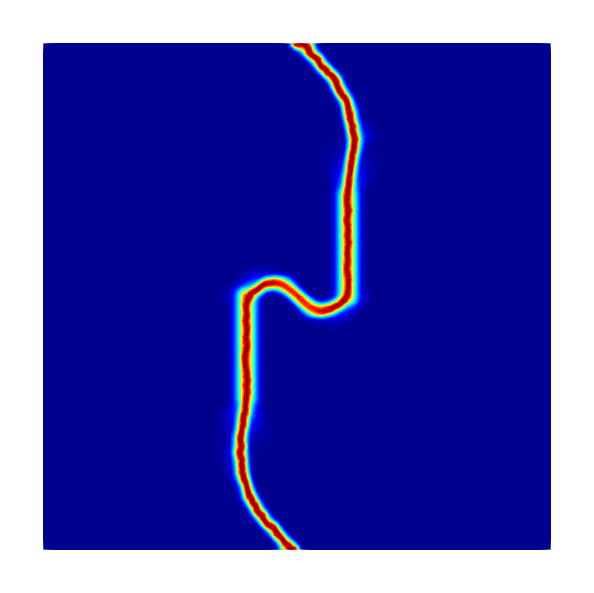
\includegraphics[width=\textwidth,scale=0.5]{Chapter4/figures/biaxial_nosplit_1.png}
    \caption{$\mathcal{D}^* = 0.14$}
    \label{fig: Chapter4/biaxial_nosplit_1}
  \end{subfigure}
  \hspace{0.03\textwidth}
  \begin{subfigure}[b]{0.23\textwidth}
    \centering
    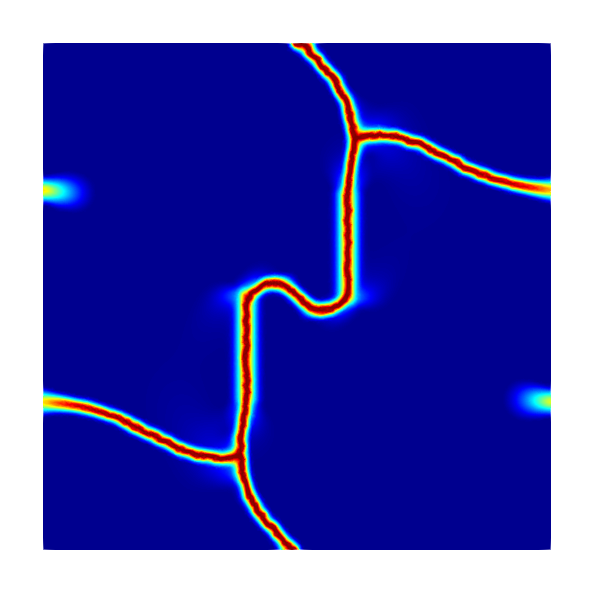
\includegraphics[width=\textwidth,scale=0.5]{Chapter4/figures/biaxial_nosplit_2.png}
    \caption{$\mathcal{D}^* = 0.19$}
    \label{fig: Chapter4/biaxial_nosplit_2}
  \end{subfigure}
  \hspace{0.03\textwidth}
  \begin{subfigure}[b]{0.23\textwidth}
    \centering
    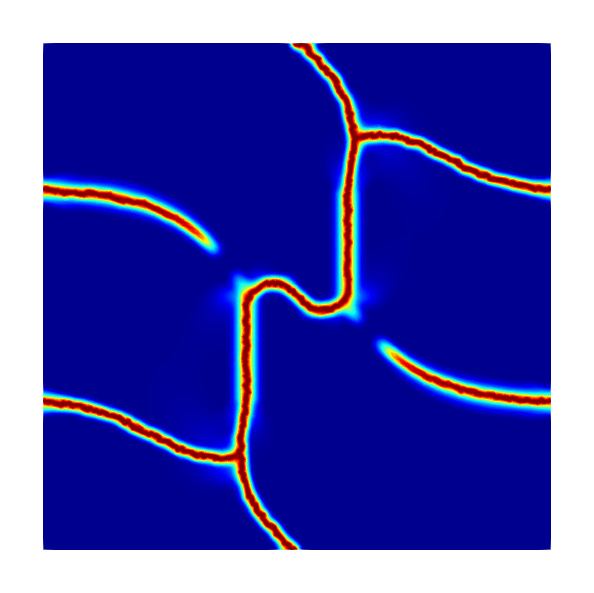
\includegraphics[width=\textwidth,scale=0.5]{Chapter4/figures/biaxial_nosplit_3.png}
    \caption{$\mathcal{D}^* = 0.75$}
    \label{fig: Chapter4/biaxial_nosplit_3}
  \end{subfigure}
  \begin{subfigure}[b]{0.065\textwidth}
    \centering
    \caption*{d}
    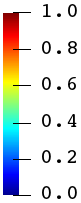
\includegraphics[width=\textwidth]{Chapter4/figures/jet_vertical.png}
    \vspace{0.15in}
  \end{subfigure}

  \begin{subfigure}[b]{0.23\textwidth}
    \centering
    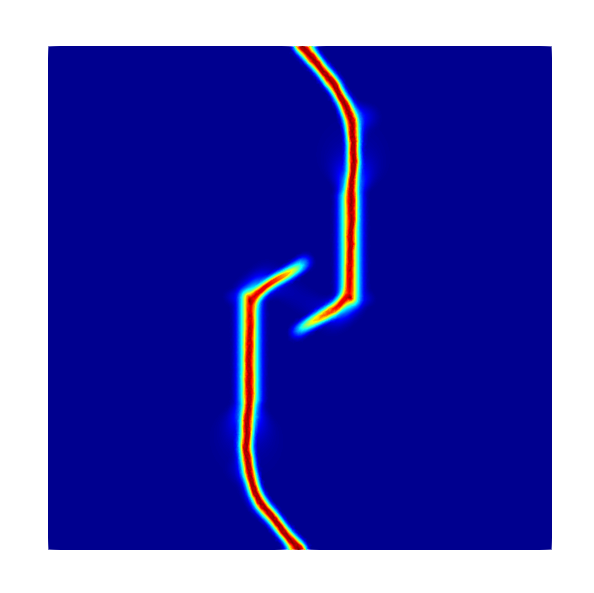
\includegraphics[width=\textwidth,scale=0.5]{Chapter4/figures/biaxial_spectral_1.png}
    \caption{$\mathcal{D}^* = 0.14$}
    \label{fig: Chapter4/biaxial_spectral_1}
  \end{subfigure}
  \hspace{0.03\textwidth}
  \begin{subfigure}[b]{0.23\textwidth}
    \centering
    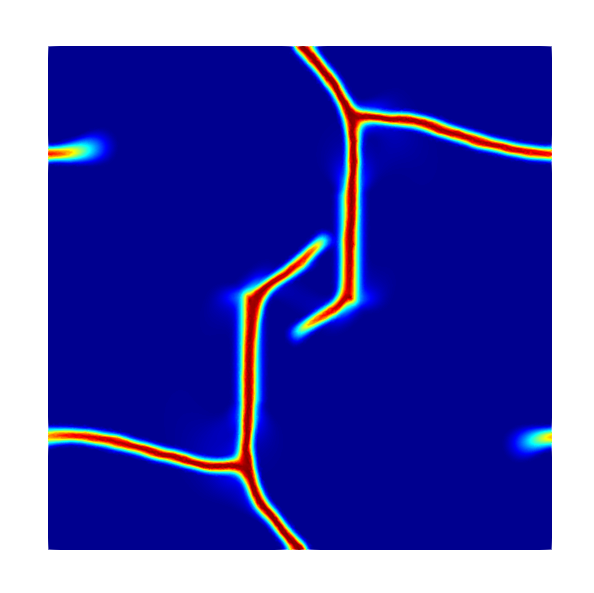
\includegraphics[width=\textwidth,scale=0.5]{Chapter4/figures/biaxial_spectral_2.png}
    \caption{$\mathcal{D}^* = 0.19$}
    \label{fig: Chapter4/biaxial_spectral_2}
  \end{subfigure}
  \hspace{0.03\textwidth}
  \begin{subfigure}[b]{0.23\textwidth}
    \centering
    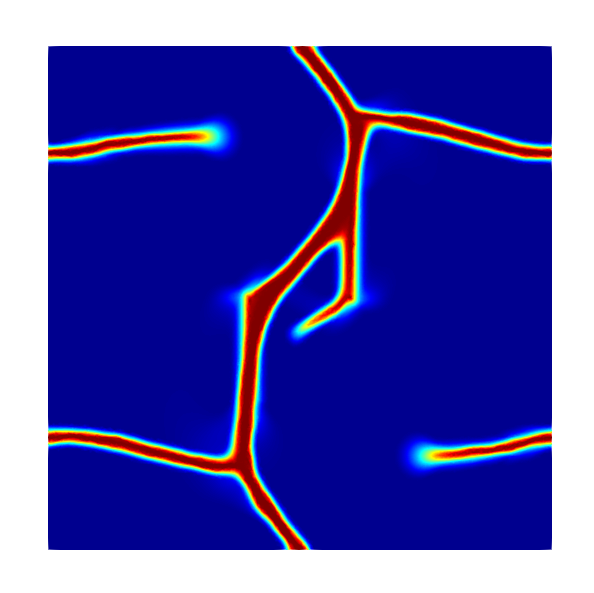
\includegraphics[width=\textwidth,scale=0.5]{Chapter4/figures/biaxial_spectral_3.png}
    \caption{$\mathcal{D}^* = 0.75$}
    \label{fig: Chapter4/biaxial_spectral_3}
  \end{subfigure}
  \begin{subfigure}[b]{0.065\textwidth}
    \centering
    \caption*{d}
    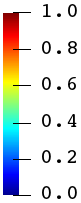
\includegraphics[width=\textwidth]{Chapter4/figures/jet_vertical.png}
    \vspace{0.15in}
  \end{subfigure}

  \begin{subfigure}[b]{0.23\textwidth}
    \centering
    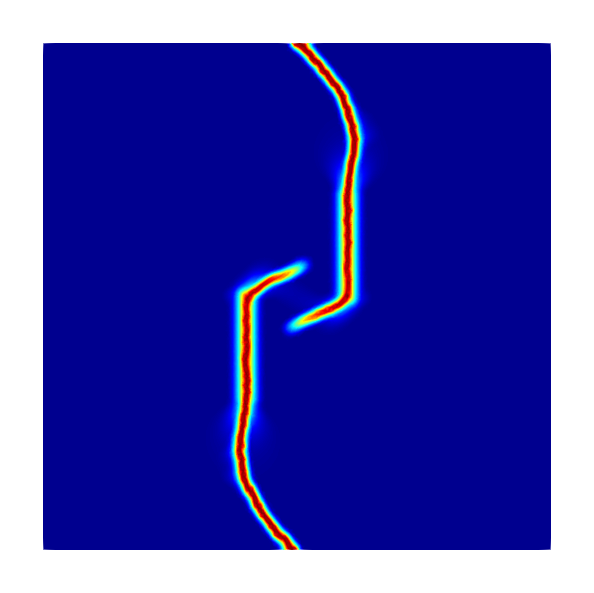
\includegraphics[width=\textwidth,scale=0.5]{Chapter4/figures/biaxial_odd_1.png}
    \caption{$\mathcal{D}^* = 0.14$}
    \label{fig: Chapter4/biaxial_odd_1}
  \end{subfigure}
  \hspace{0.03\textwidth}
  \begin{subfigure}[b]{0.23\textwidth}
    \centering
    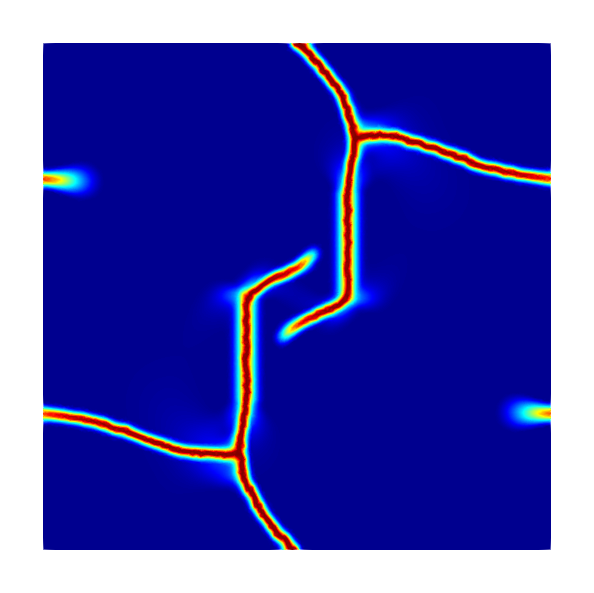
\includegraphics[width=\textwidth,scale=0.5]{Chapter4/figures/biaxial_odd_2.png}
    \caption{$\mathcal{D}^* = 0.19$}
    \label{fig: Chapter4/biaxial_odd_2}
  \end{subfigure}
  \hspace{0.03\textwidth}
  \begin{subfigure}[b]{0.23\textwidth}
    \centering
    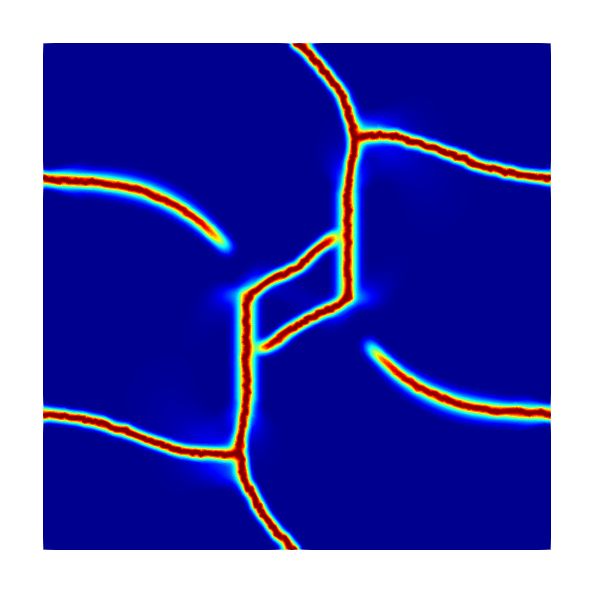
\includegraphics[width=\textwidth,scale=0.5]{Chapter4/figures/biaxial_odd_3.png}
    \caption{$\mathcal{D}^* = 0.75$}
    \label{fig: Chapter4/biaxial_odd_3}
  \end{subfigure}
  \begin{subfigure}[b]{0.065\textwidth}
    \centering
    \caption*{d}
    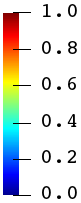
\includegraphics[width=\textwidth]{Chapter4/figures/jet_vertical.png}
    \vspace{0.15in}
  \end{subfigure}
  \caption{Crack paths obtained using (a-c) a no-split technique (d-f) the spectral decomposition (g-i) the contact split. }
  \label{fig: Chapter4/biaxial_crack_path}
\end{figure}


The no-split approach treats the entire strain energy as an active potential to be degraded, neglecting the tension-compression asymmetry. It is widely used in calculations of drying processes because the effective loading condition is assumed to be tensile: biaxial tension in 2D and triaxial tension in 3D. However, we note that tensile loading conditions do not necessarily lead to a tensile local stress/strain state everywhere in the domain, hence it is possible to have crack propagation under compression, as can be observed  in this example.   We will return to this issue after examining the results obtained using a spectral decomposition and a spectral decomposition with the contact split.

The spectral decomposition prevents crack propagation under compression (\Cref{fig: Chapter4/biaxial_spectral_1}), but without enforcing the traction-free condition on the crack surfaces represented by the phase field, which may affect secondary crack paths that emerge from existing crack surfaces (\Cref{fig: Chapter4/biaxial_spectral_2,fig: Chapter4/biaxial_spectral_2}).
Such artifacts can be removed by enforcing the traction-free condition on the regularized crack surfaces using the contact split (\Cref{fig: Chapter4/biaxial_odd_1,fig: Chapter4/biaxial_odd_2,fig: Chapter4/biaxial_odd_3}).

\begin{figure}[htb!]
  \centering
  \begin{subfigure}[b]{0.35\textwidth}
    \centering
    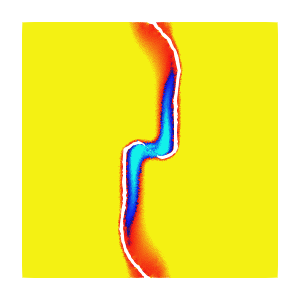
\includegraphics[width=\textwidth]{Chapter4/figures/biaxial_nosplit_stress.png}
  \end{subfigure}
  \begin{subfigure}[b]{0.15\textwidth}
    \centering
    \caption*{$\xnormal \cdot \stress \cdot \xnormal (\SI{}{\mega\pascal})$}
    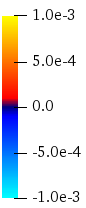
\includegraphics[width=0.7\textwidth]{Chapter4/figures/coldhot_pressure.png}
    \vspace{0.1in}
  \end{subfigure}
  \caption[Contour plot of the normal pressure right before the bridge forms.]{Contour plot of the normal pressure right before the bridge forms. The pressure is calculated for an orientation that is estimated to be orthogonal to the bridge. Elements within the contour of $d = 0.75$ are removed to indicate the current crack set. }
  \label{fig: Chapter4/biaxial_nosplit_stress}
\end{figure}


We now return to the issue of the possibility of crack growth under compression with a no-split approach.  Comparing the damage profiles shown in \Cref{fig: Chapter4/biaxial_nosplit_1,fig: Chapter4/biaxial_spectral_1,fig: Chapter4/biaxial_odd_1}
one can observe that a damage bridge forms between the two vertical initial cracks only for the case of a no-split method.  To explore this region more precisely, we consider the fields immediately before the bridge forms, and examine contour plots of the normal pressure for an orientation that is orthogonal to the bridge (\Cref{fig: Chapter4/biaxial_nosplit_stress}). The contour plots clearly indicate that the region is loaded in compression immediately before the bridge forms.

As a final observation in this section, we note that the crack-paths obtained using the spectral decomposition exhibit a broadening of the phase field at late stages of growth (\Cref{fig: Chapter4/biaxial_spectral_3}).  By contrast, the contact decomposition results in damage profiles that remain relatively thin compared to the specimen dimensions (\Cref{fig: Chapter4/biaxial_odd_3}).
